\documentclass[aspectratio=1610]{beamer}

\usetheme{unnslides}
\usefonttheme{professionalfonts}

\usepackage{listings}
\usepackage{graphicx}
\usepackage{caption}
\usepackage{cmbright}
\usepackage{fontspec}
\usepackage{unicode-math}
\usepackage{amsfonts}
\usepackage{subfig}
\usepackage{tikz}

\captionsetup[subfigure]{labelformat=empty}
\captionsetup[figure]{labelformat=empty}

\setromanfont{CMU Serif}
%\setsansfont{CMU Sans Serif}
\setmathfont{Latin Modern Math}
\setlength{\tabcolsep}{1pt}

\usepackage{polyglossia}
%\setbeamertemplate{itemize item}{\color{black}$\blacktriangleright$}

\DeclareMathOperator*{\argmax}{arg\,max}
\DeclareMathOperator*{\argmin}{arg\,min}
\DeclareMathOperator{\sign}{sign}
\DeclareMathOperator{\re}{Re}

\graphicspath{ {../images/}{img/} }

%set pages numeration
\newcommand\numbered{\setbeamertemplate{footline}{%
  \vspace{-10em}
   \raisebox{5pt}{\makebox[\paperwidth]{%
     \hfill\makebox[10pt]{%
       \usebeamerfont{footline}\usebeamercolor[fg]{footline}
       \insertframenumber}}}}}
\newcommand\unnumbered{\setbeamertemplate{footline}{}}

\title{Comparison Of Several Sequential And Parallel Derivative-free Global Optimization Algorithms}
\author{\underline{\textbf{Vladislav~Sovrasov}} and \textbf{Semen~Bevzuk}}
\institute{Lobachevsky State University of Nizhni Novgorod}
\date{}

\begin{document}
\numbered
{
\unnumbered
\begin{frame}[noframenumbering,plain]
\titlepage
\end{frame}
}

\begin{frame}
  \frametitle{Problem statement}
  \begin{columns}
    \begin{column}{0.5\textwidth}
      \begin{displaymath}
        \begin{array}{cr}\\
          \varphi(y^*)=\min\{\varphi(y):y\in D\}, \\
          D=\{y\in \mathbb{R}^N:a_i\leq y_i\leq{b_i}, 1\leq{i}\leq{N}\}
        \end{array}
      \end{displaymath}
      \(\varphi(y)\) is multiextremal objective function, which satisfies the Lipschitz condition:
      \begin{displaymath}
        |\varphi(y_1)-\varphi(y_2)|\leq L\Vert y_1-y_2\Vert,y_1,y_2\in D,
      \end{displaymath}
      where \(L>0\) is the Lipschitz constant, and \(||\cdot||\) denotes \(l_2\) norm in \(\mathbb{R}^N\)
      space.
    \end{column}
    \begin{column}{0.5\textwidth}
      \centerline{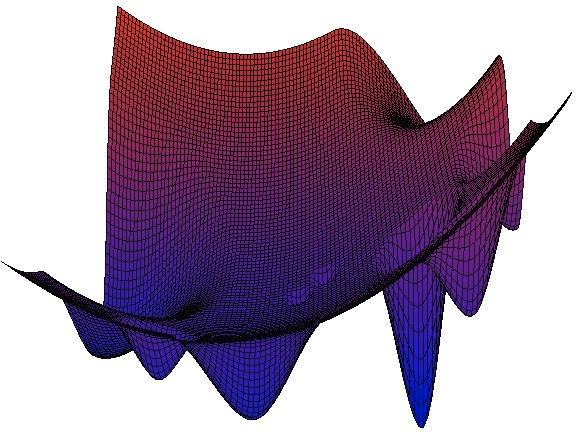
\includegraphics[width=0.9\textwidth]{img/gkls.png}}
    \end{column}
  \end{columns}
\end{frame}

\begin{frame}
  \frametitle{Methods}
  \begin{itemize}
    \item[$\square$] \textbf{Deteriminstic}:
    \begin{itemize}
      \item Have complicated internal structure in multidimensional case;
      \item Usually store and use the whole history of trials accumulated during search;
      \item Require non-trivial parallelization schemes;
      \item Under some assumptions convergence to the global solution is guaranteed.
    \end{itemize}
    \item[$\square$] \textbf{Stochastic}:
    \begin{itemize}
      \item Have relative simple internal structure;
      \item Require constant amount of memory to store internal state of some random process or individuals of population;
      \item In most cases allows wide-scale parallelization by trials or by running many copies of the same method
      with different seeds in parallel.
      \item Convergence is guaranteed in probabilistic sense only.
    \end{itemize}
  \end{itemize}
\end{frame}

\begin{frame}
  \frametitle{Methods}
  In this work considered the following solvers available in open-source:
  \begin{itemize}
    \item[$\square$] \textbf{Deteriminstic}:
    \begin{itemize}
      \item DIRECT, DIRECT$l$;
      \item AGS, AGS$l$.
    \end{itemize}
    \item[$\square$] \textbf{Stochastic}:
    \begin{itemize}
      \item Multi Level Single Linkage;
      \item StoGO;
      \item Differential Evolution;
      \item Controlled Random Search;
      \item Dual Simulated Annealing;
      \item Ant Colony Optimization.
    \end{itemize}
  \end{itemize}
\end{frame}

\begin{frame}
  \frametitle{Test problems}
  \begin{columns}
    \begin{column}{0.5\textwidth}
      Generator GKLS was employed to construct 8 sets of 100 test problems:
      \begin{displaymath}
        \begin{matrix}
          f(x)=
          \left\{
          \begin{matrix}
          C_i(x), x \in S_i, i\in 2,\dots ,m \\
          \Vert x-T \Vert^2 + t, x\not\in S_2,\dots,S_m
          \end{matrix} \right.
        \end{matrix}
      \end{displaymath}

      The generator allows to adjust:
      \begin{itemize}
        \item the number of local minimas;
        \item the size of the global minima attraction region;
        \item the space dimension.
      \end{itemize}
    \end{column}
    \begin{column}{0.5\textwidth}
      \centerline{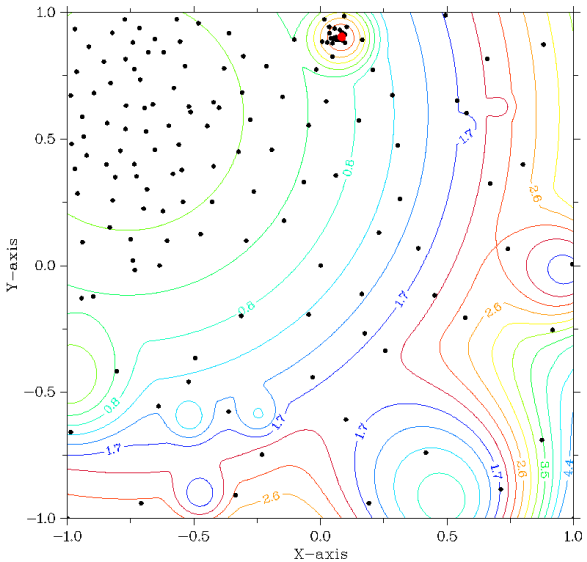
\includegraphics[width=0.9\textwidth]{gkls_color.png}}
    \end{column}
  \end{columns}
\end{frame}

\begin{frame}
  \frametitle{Results of sequential methods}

  \begin{table}
  \begin{center}
  \caption{Averaged number of trials executed by sequential methods for solving the test
  optimization problems}
  \resizebox{\textwidth}{!}{%
    \begin{tabular}{|l|{c}|{c}|{c}|{c}|{c}|{c}|{c}|{c}|{c}|{c}|}
      \hline
      & AGS & AGS\(l\) & CRS & DIRECT & DIRECT\(l\) & MLSL & SDA & DE & StoGO \\
    \hline
    \(F_{GR}\)     & 193.1 &  \textbf{158.3} & 400.3 & 182.3 & 214.9 & 947.2 & 691.2 & 1257.3 &
  1336.8 \\
    \hline
    GKLS 2d Simple &  254.9 & 217.6 & 510.6 & \textbf{189.0} & 255.2 & 556.8 & 356.3 & 952.2
  & 1251.5 \\
    \hline
    GKLS 2d Hard   &  728.7 & \textbf{488.0} & 844.7 & 985.4 & 1126.7 & 1042.5 & 1637.9 &
  1041.1 & 2532.2 \\
    \hline
    GKLS 3d Simple &  1372.1 & 1195.3 & 4145.8 & \textbf{973.6} & 1477.8 & 4609.2 & 2706.5 &
  5956.94 & 3856.1 \\
    \hline
    GKLS 3d Hard   &  3636.1 & \textbf{1930.5} & 6787.0 & 2298.7 & 3553.3 & 5640.1 & 4708.4 &
  6914.3 & 7843.2 \\
    \hline
    GKLS 4d Simple &  26654.1 & 11095.7 & 37436.8 & \textbf{7824.3} & 15994.1 & 41514.3 &
  21417.9 & 19157.7 & 59895.4 \\
    \hline
    GKLS 4d Hard   &  54536.8 &  \textbf{23167.8} &  73779.3 &  23204.4 &  54489.9 &  80247.2
  &  68815.5 &  27466.1 &  109328.1  \\
    \hline
    GKLS 5d Simple &  29810.0 & 11529.0 & 143575.0 & \textbf{7166.5} & 13970.5 & 52647.6 &
  34255.3 & 73074.5 & 91580.4 \\
    \hline
    GKLS 5d Hard   &  113129.1 & 67652.7 & 165192.8 & \textbf{66327.4} & 164390.6 & 138766.2
  & 116973.1 & 105496.9 & 155123.8 \\
    \hline
  \end{tabular}}
    \label{tab:trials}
  \end{center}
  \end{table}
\end{frame}

\begin{frame}
  \frametitle{Results of sequential methods}
  \begin{table}
  \begin{center}
  \caption{Number of test optimization problems solved by sequential methods}
    \begin{tabular}{|l|{c}|{c}|{c}|{c}|{c}|{c}|{c}|{c}|{c}|{c}|}
      \hline
      & AGS & AGS\(l\) & CRS & DIRECT & DIRECT\(l\) & MLSL & SDA & DE & StoGO \\
    \hline
    \(F_{GR}\)     &  100 & 100 & 76  & 100 & 100 & 97  & 96  & 96  & 67\\
    \hline
    GKLS 2d Simple &  100 & 100 & 85  & 100 & 100 & 100 & 100 & 98  & 90\\
    \hline
    GKLS 2d Hard   &  100 & 100 & 74  & 100 & 100 & 100 & 93  & 85  & 77 \\
    \hline
    GKLS 3d Simple &  100 & 97  & 75  & 100 & 100 & 100 & 89  & 86  & 44 \\
    \hline
    GKLS 3d Hard   &  100  & 99   & 72   & 100  & 99   & 100  & 88   & 77   & 43 \\
    \hline
    GKLS 4d Simple &  100 & 100 & 46  & 100 & 100 & 94  & 78  & 59  & 16 \\
    \hline
    GKLS 4d Hard   &  100 & 100 & 47  & 99  & 97  & 94  & 72  & 32  & 10  \\
    \hline
    GKLS 5d Simple &  100 & 100 & 68  & 100 & 100 & 98  & 100 & 77  & 9  \\
    \hline
    GKLS 5d Hard   &  97  & 99  & 42  & 100 & 90  & 79  & 84  & 48  & 8 \\
    \hline
    \end{tabular}
    \label{tab:solved}
  \end{center}
  \end{table}
\end{frame}

\begin{frame}
  \frametitle{Univariate Algorithm of Global Search}
  Optimization method generates search sequence \(\{x_k\}\) and consists of the following steps:
  \begin{enumerate}
    \setlength{\itemindent}{.1in}
    \item[Step 1.] Sort the search information (one-dimensional points) in increasing order.
    \item[Step 2.] For each interval \((x_{i-1}, x_i)\) compute quantity \(R(i)\), called characteristic.
    \item[Step 3.] Choose \(p\) intervals \((x_{t_j-1}, x_{t_j})\) with the greatest characteristics and
    compute objective \(\varphi(y(x^{k+j}))\) in points chosen using the decision rule \(d\):
    \begin{displaymath}
      x^{k+1+j}=d(t)\in (x_{t_j-1}, x_{t_j}),\:j=\overline{1,p}
    \end{displaymath}
    \item[Step 4.] If \(x_{t_j}-x_{t_j-1}<\varepsilon\) for one of \(j=\overline{1,p}\), stop the method.
  \end{enumerate}
  \textit{\footnotesize	{Detailed description: Strongin R.G., Sergeyev Ya.D.: Global optimization with non-convex constraints. Sequential and parallel algorithms (2000), Chapter 7}}
\end{frame}

\begin{frame}
  \begin{center}
  \frametitle{Dimension reduction}
  Peano-type curve \(y(x)\) allows to reduce the dimension of the original problem:
  \begin{gather}
    \lbrace y\in \mathbb{R}^N:-2^{-1}\leqslant y_i\leqslant 2^{-1},1\leqslant i\leqslant N\rbrace=\{y(x):0\leqslant x\leqslant 1\} \nonumber \\
    \min\{\varphi(y): y\in D\}=\min\{\varphi(y(x)): x\in [0,1]\} \nonumber
  \end{gather}
  \(y(x)\) is non-smooth function which continuously maps the segment \([0,1]\) to the hypercube \(D\).
  \begin{figure}[ht]
    \vspace*{-0.5cm}
    \subfloat{{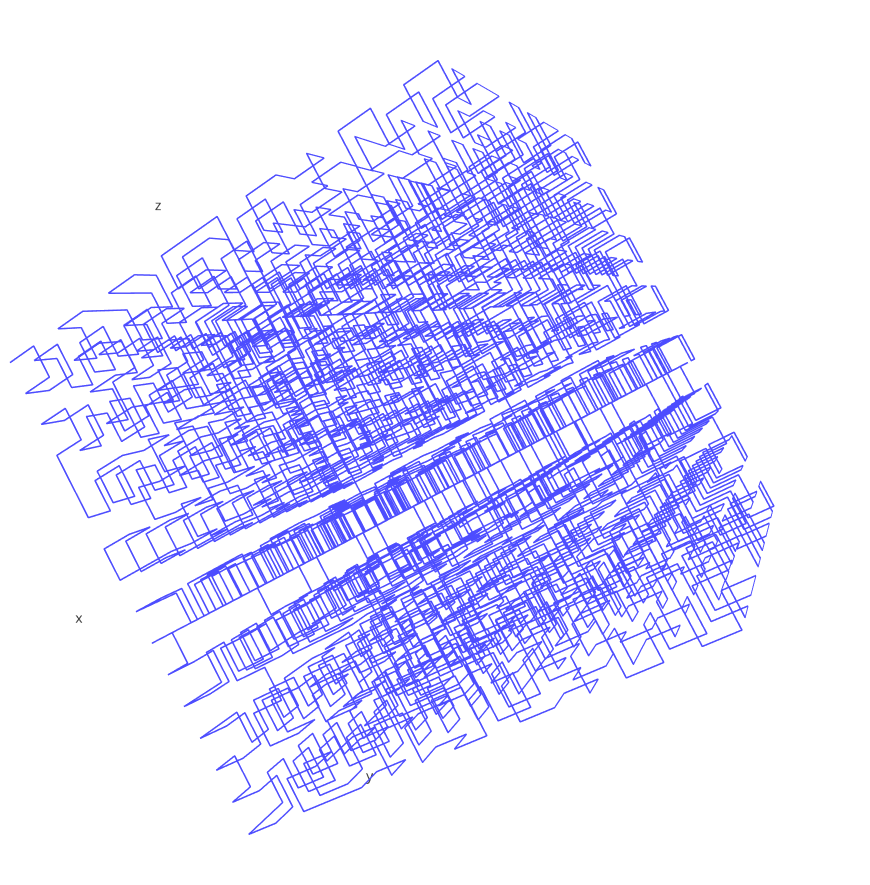
\includegraphics[width=.35\textwidth]{peano3d.png} }}
    \subfloat{{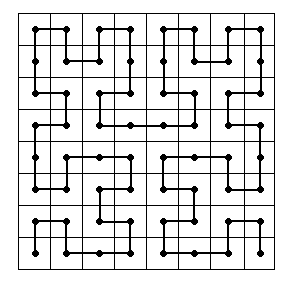
\includegraphics[width=.35\textwidth]{peano2d.png} }}
  \end{figure}
\end{center}
\end{frame}

\begin{frame}
  \frametitle{Globalizer parallel solver}
  \begin{figure}[ht]
    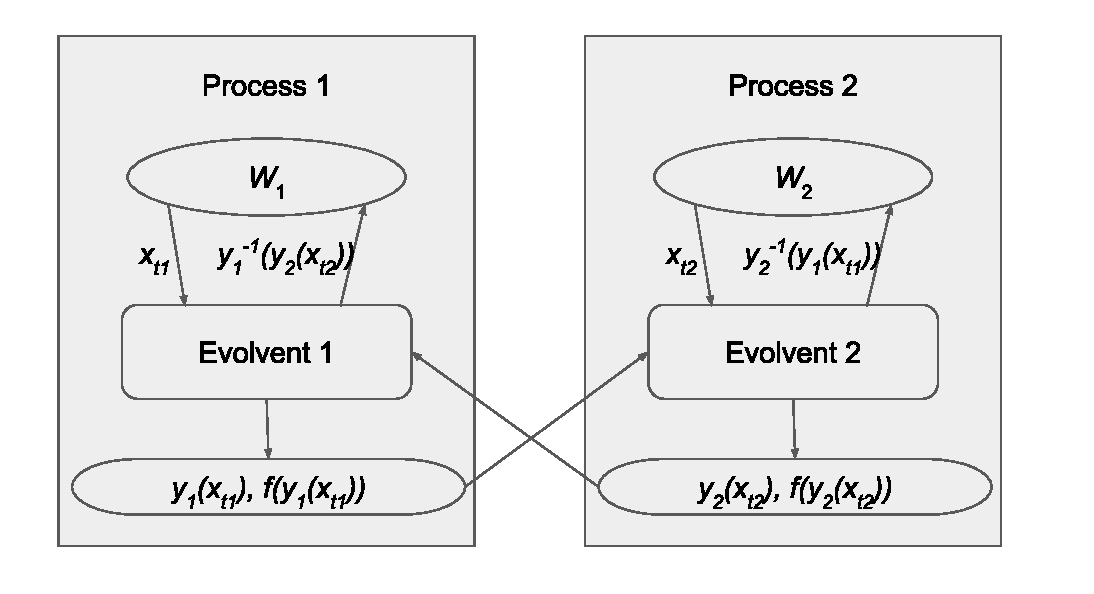
\includegraphics[width=0.95\textwidth]{evolvents_parallel.pdf}
  \end{figure}
\end{frame}

\begin{frame}
  \frametitle{MIDACO parallel solver}
  The MIDACO solver utilizes reverse communication architecture.
  Reverse communication means that the call of the objective function happens outside and
  independently of the MIDACO source code.
  Relying on this feature the following distributed parallelization scheme was implemented:
  \begin{enumerate}
    \item MIDACO runs at the master node and generates \(n \times p\) new trial points at each
  iteration.
    \item Each of \(n\) distributed computational nodes gets \(p\) points from the master and performs
  \(p\) parallel trials on local computing devices.
    \item Each of \(n\) distributed computational nodes sends \(p\) values of the objective function to
  the master.
  \end{enumerate}

  In this scheme all distributed communications were implemented using the MPI library.
  Parallelism within a single node is powered by the OpenMP standard.
\end{frame}

\begin{frame}
  \frametitle{Cluster environment}
  \begin{center}
  The computational experiments have been carried out on the Lobachevsky supercomputer at  State University of Nizhni Novgorod.
  One node includes 2 Intel Sandy Bridge E5-2660 2.2 GHz processors and 64 GB RAM.

  Each node runs under CentOS 7 Linux with GCC 4.8 compiler and Intel MPI library.
\end{center}
\end{frame}

\begin{frame}
  \frametitle{Results of the parallel algorithms}
  \begin{table}
    \centering
    \caption{Averaged numbers of iterations executed by the parallel algorithms for solving the test
  optimization problems}
    \label{tab:iterations}
    \begin{tabular}{cccccccc}
      \cline{3-8}\noalign{\smallskip}
      \multicolumn{2}{c}{  } & \textit{p} & \multicolumn{2}{c}{Globalizer} & &
  \multicolumn{2}{c}{MIDACO}   \\
      \noalign{\smallskip} \cline{4-5} \cline{7-8}  \noalign{\smallskip}
      \multicolumn{2}{c}{  } & & \textit{Simple} & \textit{Hard} & & \textit{Simple} &
  \textit{Hard}  \\
      \noalign{\smallskip}\hline
      I & \textbf{1 cluster node}
        & \textit{1} &   25270 (100)  & 55180 (99) & & 27645 (98) & 72068 (71)  \\
      &  & \textit{16} & 1765 (100)  & 3714 (100) & &  1640 (97) & 4304 (70) \\
      \hline \noalign{\smallskip}
  II  & \textbf{2 cluster nodes}  %\multirow{3}{*}{}
    & \textit{1} & 13056 (100) & 22938 (99) & & 10558 (89) & 27128 (73) \\
  &   & \textit{16} & 732 (100) & 1759 (100)  &  & 1130 (92) & 2254 (73) \\
      \hline \noalign{\smallskip}
  III & \textbf{4 cluster nodes} %\multirow{3}{*}{}
    & \textit{1}  & 5016 (100) & 12703 (100) & & 5777 (94) & 15980 (75) \\
  & & \textit{16} & 367 (100) & 776 (100) & & 529 (88) &  1264 (66) \\
      \hline \noalign{\smallskip}
  VI & \textbf{8 cluster nodes} %\multirow{3}{*}{}
    & \textit{1}  & 2103 (100) & 5063 (100) & & 2847 (97) & 9853 (83)\\
  & & \textit{16} & 145 (100)  & 310 (100)  & & 272 (83) & 774 (57)\\
      \hline \noalign{\smallskip}
  V & \textbf{12 cluster nodes} %\multirow{3}{*}{}
    & \textit{1}  & 1155 (100) & 2399 (100) & & 2233 (98) & 6022 (86) \\
  & & \textit{16} & 76 (100)  & 159 (100)  & & 168 (87) & 393 (53)\\
      \noalign{\smallskip}\hline
    \end{tabular}
  \end{table}
\end{frame}

\begin{frame}
  \frametitle{Results of the parallel algorithms}
  \begin{table}
    \centering
    \caption{Speedup of parallel computations executed by the parallel algorithms}
    \label{tab:speedup}
    \begin{tabular}{cccccccc}
      \cline{3-8}\noalign{\smallskip}
      \multicolumn{2}{c}{  } & \textit{p} & \multicolumn{2}{c}{Globalizer} & &
  \multicolumn{2}{c}{MIDACO}   \\
      \noalign{\smallskip} \cline{4-5} \cline{7-8}  \noalign{\smallskip}
      \multicolumn{2}{c}{  } & & \textit{Simple} & \textit{Hard} & & \textit{Simple} &
  \textit{Hard}  \\
      \noalign{\smallskip}\hline
  I  & \textbf{1 cluster node}  %\multirow{3}{*}{}
      & \textit{1}   & 25270 (27.3s) & 55180 (61.8s) & & 27645 (32.2s) & 72068 (132.5s)  \\
    &  & \textit{16} & 14.3(11.7) & 14.9(12.6)  & &  16.9(14.4) & 16.7(14.4) \\
    \hline \noalign{\smallskip}
  II  & \textbf{2 cluster nodes}  %\multirow{3}{*}{}
    & \textit{1}      &   1.9(1.9) & 2.4(2.2)  & & 2.6(1.7) & 2.7(2.3) \\
    &   & \textit{16} & 34.5(20.4) & 31.4(18.8) & & 24.5(18.8) & 32.0(29.1) \\
      \noalign{\smallskip}\hline	\noalign{\smallskip}
  III  & \textbf{4 cluster nodes}  %\multirow{3}{*}{}
  & \textit{1}      & 5.0(4.6) & 4.3(4.1) & & 4.8(3.9) & 4.5(4.4) \\
  &   & \textit{16} & 68.8(23.7) & 71.2(25.8) & & 52.3(32.9) & 57.0(50.2) \\
    \noalign{\smallskip}\hline	\noalign{\smallskip}
  VI & \textbf{8 cluster nodes} %\multirow{3}{*}{}
  & \textit{1}    & 12.0(8.7) & 10.9(8.3) & & 9.7(8.2)    & 7.3(9.0)    \\
  & & \textit{16} & 174.1(4.7) & 177.8(5.3) & & 101.6(51.6) & 93.1(84.1) \\
      \noalign{\smallskip}\hline
      V & \textbf{12 cluster nodes} %\multirow{3}{*}{}
      & \textit{1}    & 21.9(11.4)  & 23.0(12.8)  & & 12.4(11.1)  & 12.0(14.8)  \\
      & & \textit{16} & 333.5(2.7) & 347.9(3.0) & & 164.5(82.0) & 183.2(129.7) \\
          \noalign{\smallskip}\hline
    \end{tabular}
  \end{table}
\end{frame}

\begin{frame}
  \frametitle{Results of the parallel algorithms}
  \begin{figure}[ht]
    \centering
    \subfloat[$p=1$]{{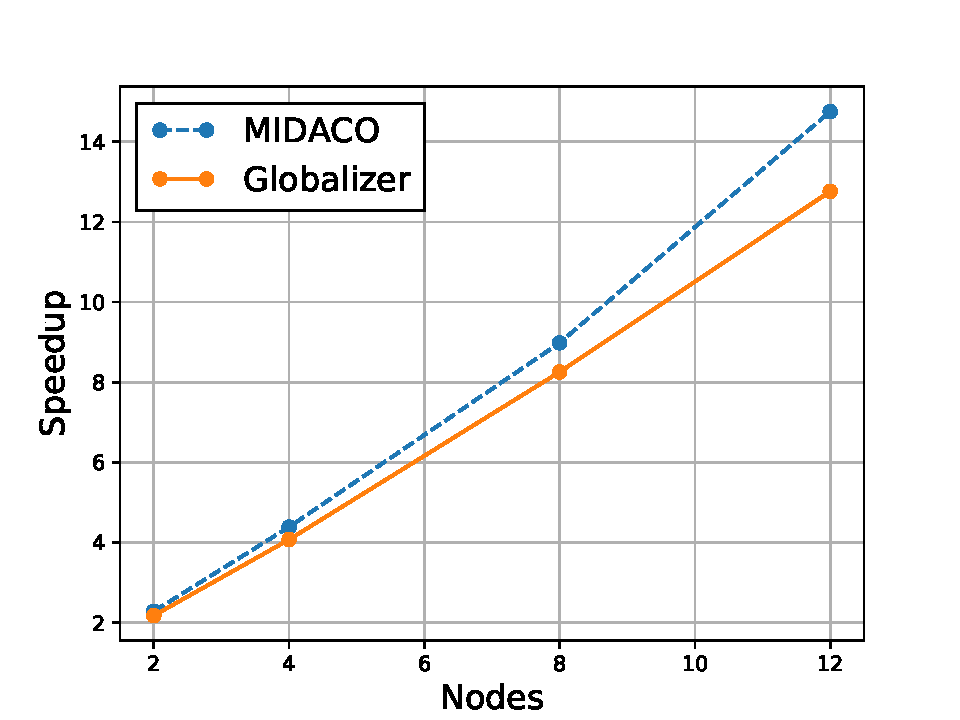
\includegraphics[width=.5\textwidth]{speedup_midaco_globalizer_p_1.pdf}}\label{fig:speedup_p1}}
    \subfloat[$p=16$]{{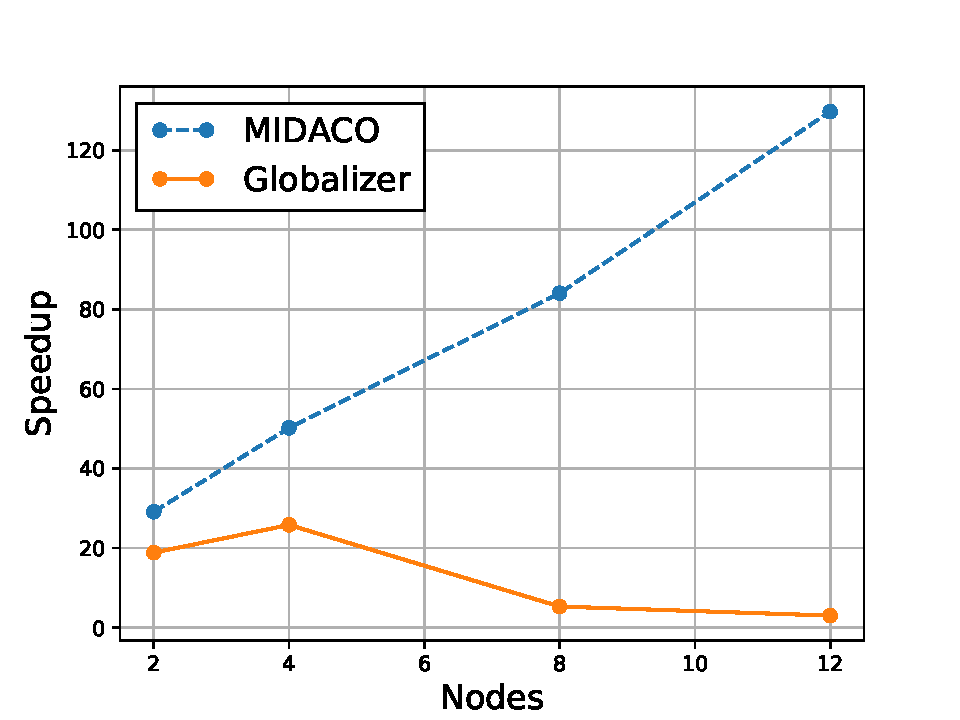
\includegraphics[width=.5\textwidth]{speedup_midaco_globalizer_p_16.pdf}}\label{fig:speedup_p16}}
    \caption{Speedup demonstrated by the parallel algorithms when solving problems from the GKLS 4d Hard class}
  \end{figure}
\end{frame}

\begin{frame}
  \frametitle{Results of the parallel algorithms}
  \begin{figure}[ht]
    \centering
    \subfloat[$p=1$]{{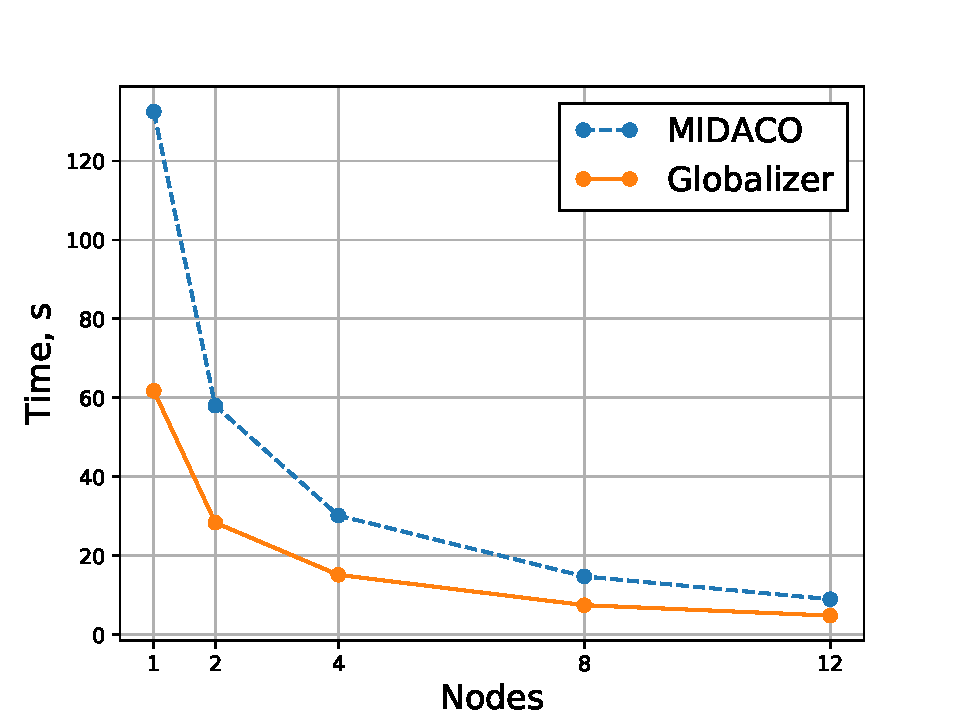
\includegraphics[width=.5\textwidth]{time_midaco_globalizer_p_1.pdf}}\label{fig:time_p1}}
    \subfloat[$p=16$]{{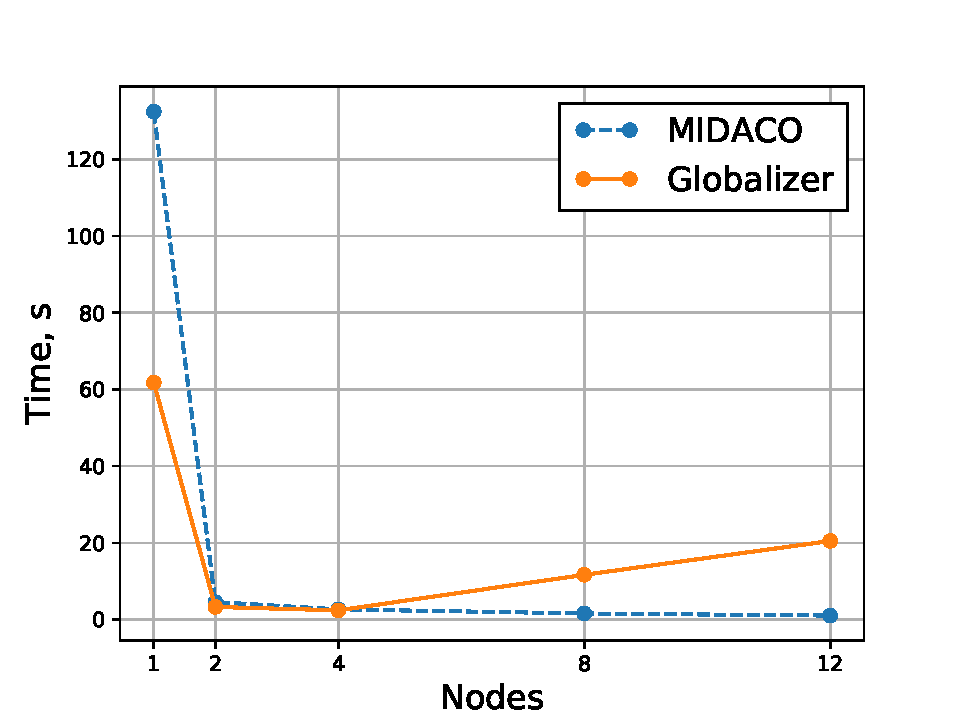
\includegraphics[width=.5\textwidth]{time_midaco_globalizer_p_16.pdf}}\label{fig:time_p16}}
    \caption{Averaged execution time of the parallel algorithms when solving problems from the GKLS 4d Hard class}
  \end{figure}
\end{frame}

\begin{frame}
  \frametitle{Conclusions}
    %Already done:
    \begin{itemize}
      \item AGS\(l\) method implemented in the Globalizer system has demonstrated the convergence
    speed and reliability at the level of DIRECT and exceeds many other algorithms, the open-source
    implementations of which are available;
    \item the stochastic optimization methods inferior to the deterministic ones in the convergence
  speed and in reliability. It is manifested especially strongly on more complex multiextremal
  problems;
    \item the parallel version of the Globalizer system demonstrates good speedup
  when running on several nodes, on each of which a single objective function value per iterations is
  computed. When solving the problems with fast computable objective functions and using multiple
  threads on the nodes, the speedup for the Globalizer system degrade with increasing
  number of nodes;
    \item the MIDACO system is the most suitable for simple global optimization problems with the
  fast-computable objective functions. In this case, MIDACO is reliable enough and provides a linear
  speedup with increasing number of nodes and threads executed on these ones in parallel.
    \end{itemize}
    %Future work:
    %\begin{itemize}
    %  \item
    %\end{itemize}
\end{frame}
{
\unnumbered
\begin{frame}{{}}
  \frametitle{Q\&A}
  \begin{center}
    \Large{Contacts:}
\vspace{0.5cm}

    sovrasov.vlad@gmail.com

    https://github.com/sovrasov
  \end{center}
\end{frame}
}
\end{document}
